\chapter{試作1号機:スマートフォン搭載ハンド}
\newpage

%ここに3章の概要(本章での背景,目的(動機),章内の節構成について言及してやると,何を述べているのか理解しやすい.
%(モバイル)ロボットハンド作製を通じ,実用化のための課題点を整理する.
\section{要求仕様}
%1章で修論全体もしくは一般的な夢物語を述べて,3章ではその達成のための布石として,必要なスペックを述べる必要がある.いきなり節から始めるのであれば,ここにその内容を再度記載しておく方が親切な気がする.

1号機では本体の基本デザイン・自律動作・携帯性に重点をおいて設計する.

ハードウェアとして自律移動が可能で物体を把持でき,また小型で携帯可能な重量が要求される.そのため,環境を認識できるセンサ,対象物に接近するためのアクチュエータ,把持を行うためのアクチュエータ,これらを制御するコンピュータが必要である.

ソフトウェアとして,センサ情報をEdgeで計算しアクチュエータ制御を行うことが要求される.また持ち運ぶため環境にロバストな制御方式であることが必要である.ただし,衝突リスク等を考慮するとアクチュエータの制御は高速に行う必要はなく,数ミリ秒毎に制御する高速動作は求められない.


\section{機構設計・機体デザイン}
環境を把握するセンサとして,簡便でかつ情報量の多いカメラを採用した.また自律移動には車輪を採用し,後輪駆動の3輪車とした.車輪の駆動にはDCモーターを用いた.把持動作にはサーボモータを使用し,1軸の握る動作を実装した.

上記の画像取得,認識,処理,アクチュエータ制御をすべてスマートフォンで実現を試みた.ロボットハンドにはスマートフォンを搭載し,スマートフォンのフロントカメラから環境を認識させた.アクチュエータの制御にはワンチップコンピュータを使用し,スマートフォンとシリアル通信を行うことで各アクチュエータをそれぞれ制御した.

これらを考慮して\fig{1号機CAD}に示すようなフレームを3DCAD(123D Design Autodesk社を使用)で設計した.また,ロボットハンドの向きは\fig{1号機向き}に示す,ソフトウェアでの画像(配列)の向きと同様の定義とした.
% 向きはここで定義する.CADの写真を使って向きを定義する.

\begin{figure}[H]
    \centering
    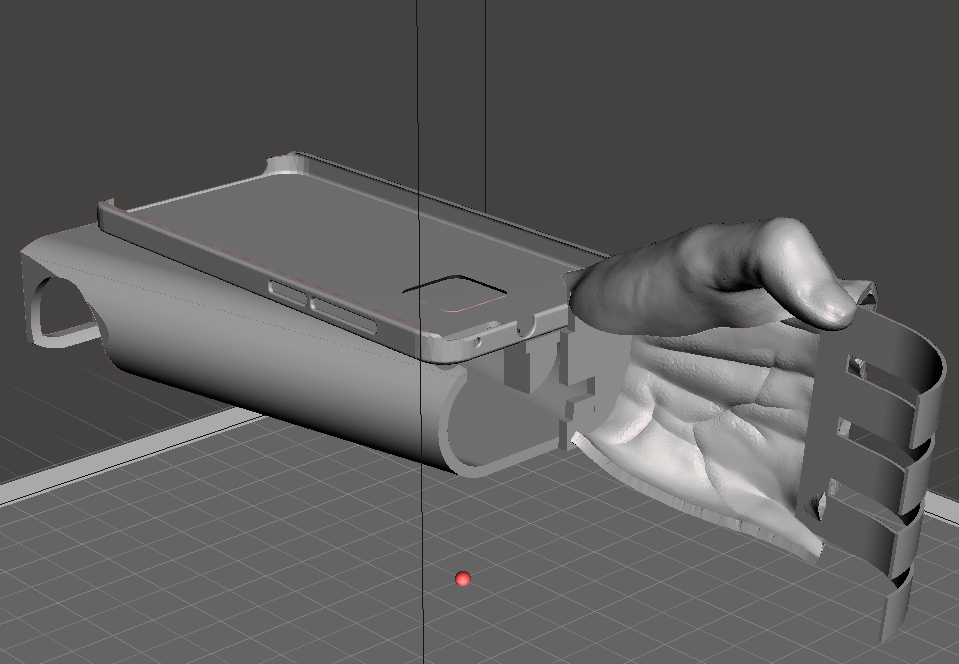
\includegraphics[width=\linewidth]{figure/chapter3/robothand-v1_cad}
    \caption{3DCAD image of prototype No.1}
    \label{fig:1号機CAD}
\end{figure}


\section{制御アルゴリズム}
自律移動のアルゴリズムは強化学習で行った.強化学習は環境に対してロバストであるため,実生活において有用だと考えた.強化学習の最適化としてはQ-Learningを用いて学習を行い,方策として$\epsilon$-greedy方策を使用した.

\fig{1号機制御図}に1号機の制御系ブロック図を示す.ロボットハンドの接近動作のフローを述べる.
まず,フロントカメラから480x640 pixelの画像を取得する.取得した画像をHSV空間に変換し,赤色だけを抽出しターゲットのマスク画像を得る.マスク画像からターゲットの面積(ピクセル数)と画像における重心を求め,面積を画像サイズで規格化した.この面積値と前フレームでの面積値との差分の2次元を状態として与えた.行動として前進,後退,右旋回,左旋回の4次元を与えた.報酬としてタスクが成功したら+1,1episode以内で成功できなかったら-1,その他では0とした.episodeの終了判定に面積値と重心座標を用いて,面積が40以上で最接近とし,また重心座標がロボットの中心座標から10pixel以内であれば正面に来たと判定した.接近が完了したらサーボモータを動かして対象物を握るようルールベース化した.

\begin{figure}[H]
    \centering
    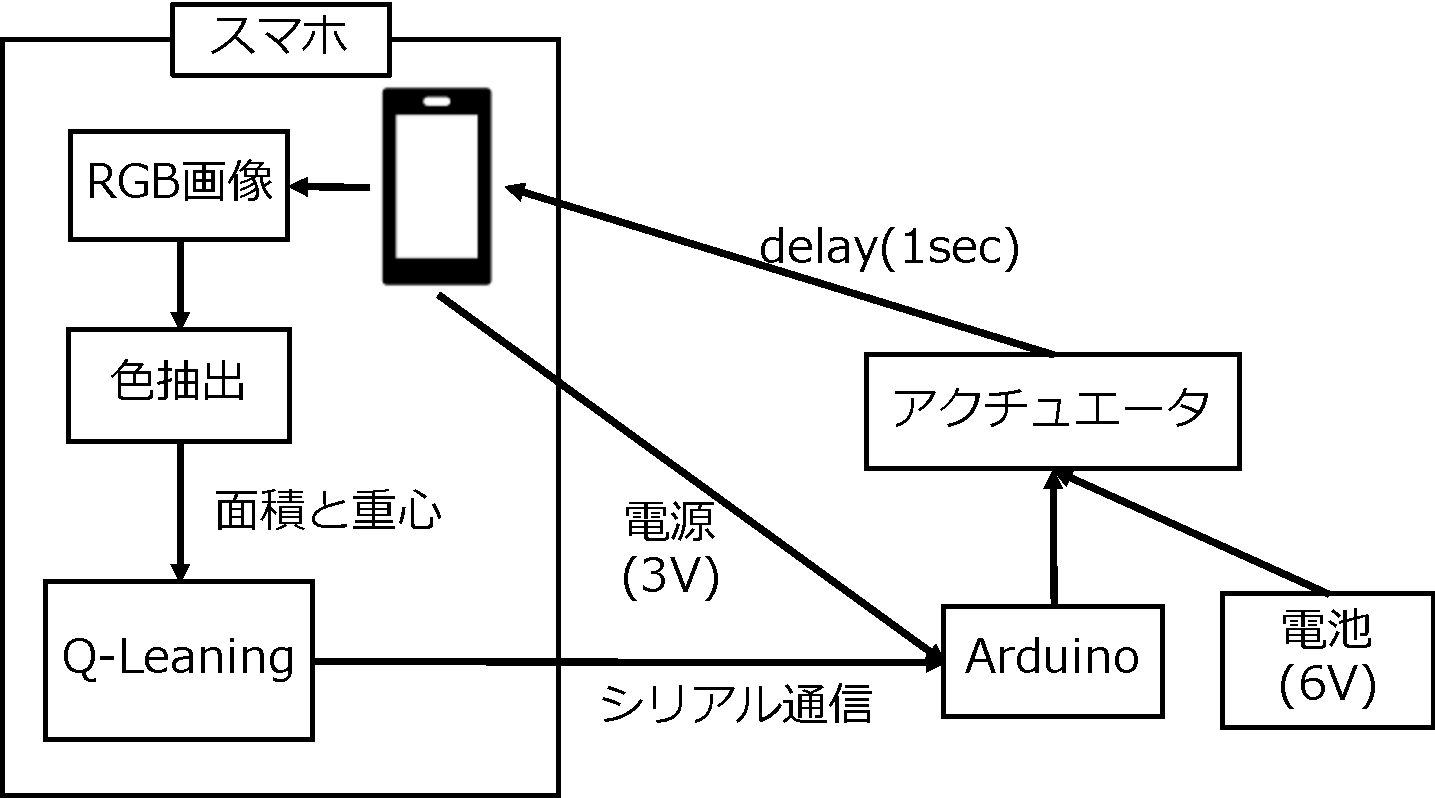
\includegraphics[width=0.7\linewidth]{figure/chapter3/1号機制御図}
    \caption{Block diagram of Prototype No.1}
    \label{fig:1号機制御図}
\end{figure}


\section{実機作製}
1号機作製にあたって使用した部品を\tab{1号機部品}まとめた.

\begin{table}[H]
    \centering
    \caption{Components of prototype No.1}
    \begin{tabular}{cc}\toprule
        本体フレーム & PLA(黒) \\
        スマートフォン & HUAWEI P10 lite \\
        DCモーター & \href{http://akizukidenshi.com/catalog/g/gM-12379/}{STLギヤモータ 栄42D長軸型} \\
        サーボモータ & \href{http://akizukidenshi.com/catalog/g/gM-01908/}{GWSサーボ MICRO/2BBMG/FP(フタバ)} \\ 
        タイヤ & \href{https://tamiya.com/japan/products/70194/index.html}{TAMIYA製スパイクタイヤ} \\ 
        コンピュータ & \href{http://akizukidenshi.com/catalog/g/gK-10347/}{ArduinoProMini} + \href{https://www.switch-science.com/catalog/1032/}{FTDI} \\ 
        バッテリー & 単4電池x4本 + 電池パック \\
        \bottomrule
    \end{tabular} 
    \label{tab:1号機部品}
\end{table}

ロボットハンドのフレームは簡便さと軽さを考慮し3Dプリンタ(TITAN GENKEI社)で造形を行った.\fig{1号機外観}に作製したロボットハンドの外観を示す.スマートフォンは腕の上部に装着し着脱ができるようにした.スマートフォンのフロントカメラに鏡を角度45度傾けてで置くことでz軸方向(スマートフォンの上側方向)を捉えることができるようにした.また,腕部分にバッテリーとタイヤ,そしてArduinoを含む回路を収め,上から見るとスマートフォンと手のみが見えるように工夫して組み立てた.1号機の総重量は473.82 gであった.

\begin{figure}
    \centering
    \begin{minipage}{\linewidth}
        \centering
        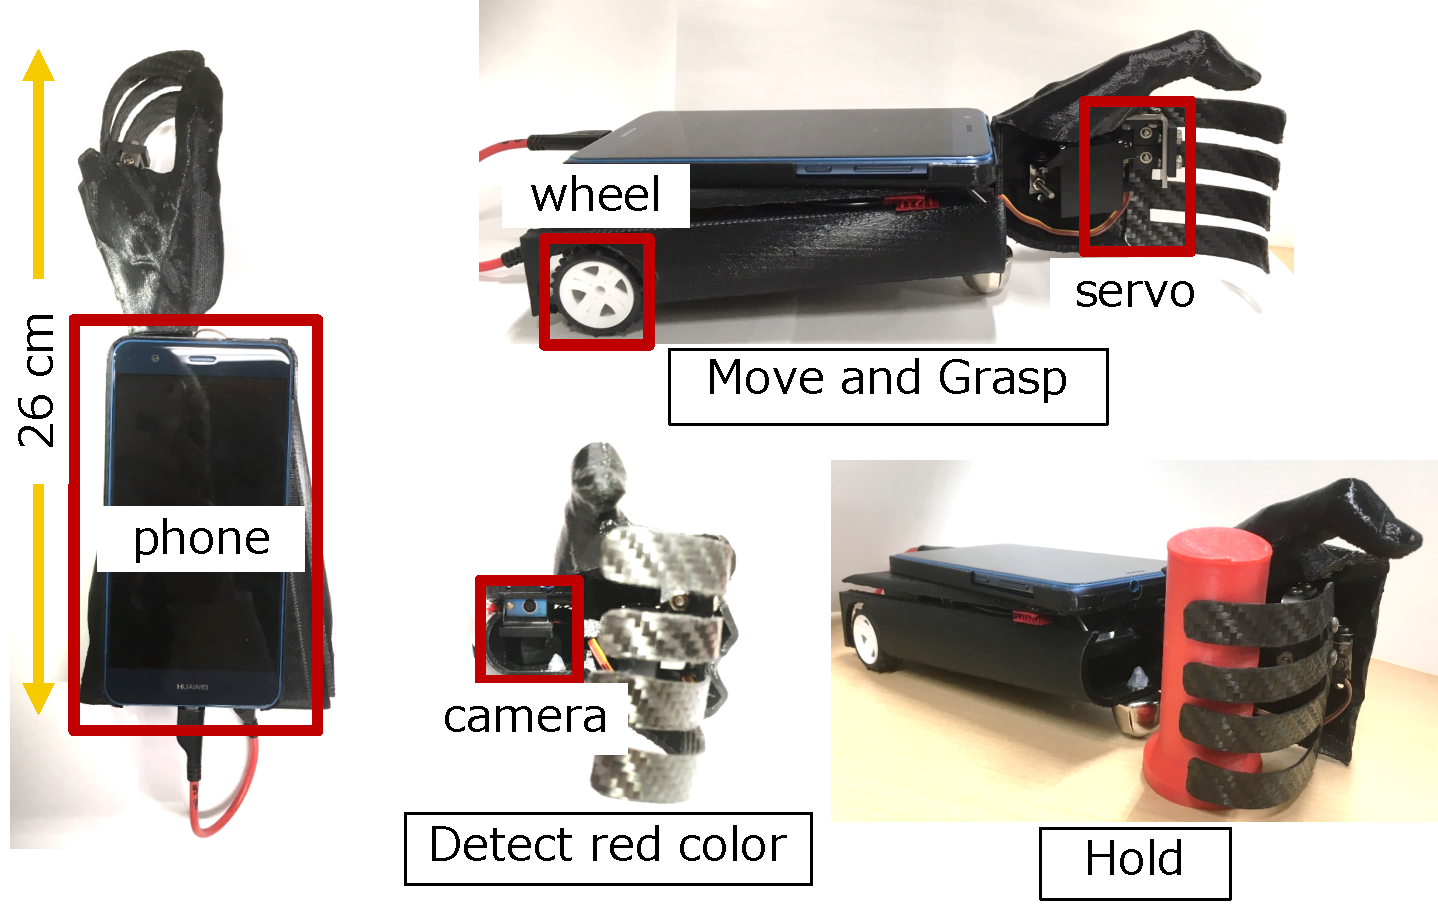
\includegraphics[width=\linewidth]{figure/chapter3/1号機外観}
        \caption{Appearance of prototype No.1 made of 3D printer. Weight is 473.82 g.}
        \label{fig:1号機外観}
    \end{minipage}
    \begin{minipage}{\linewidth}
        \centering
        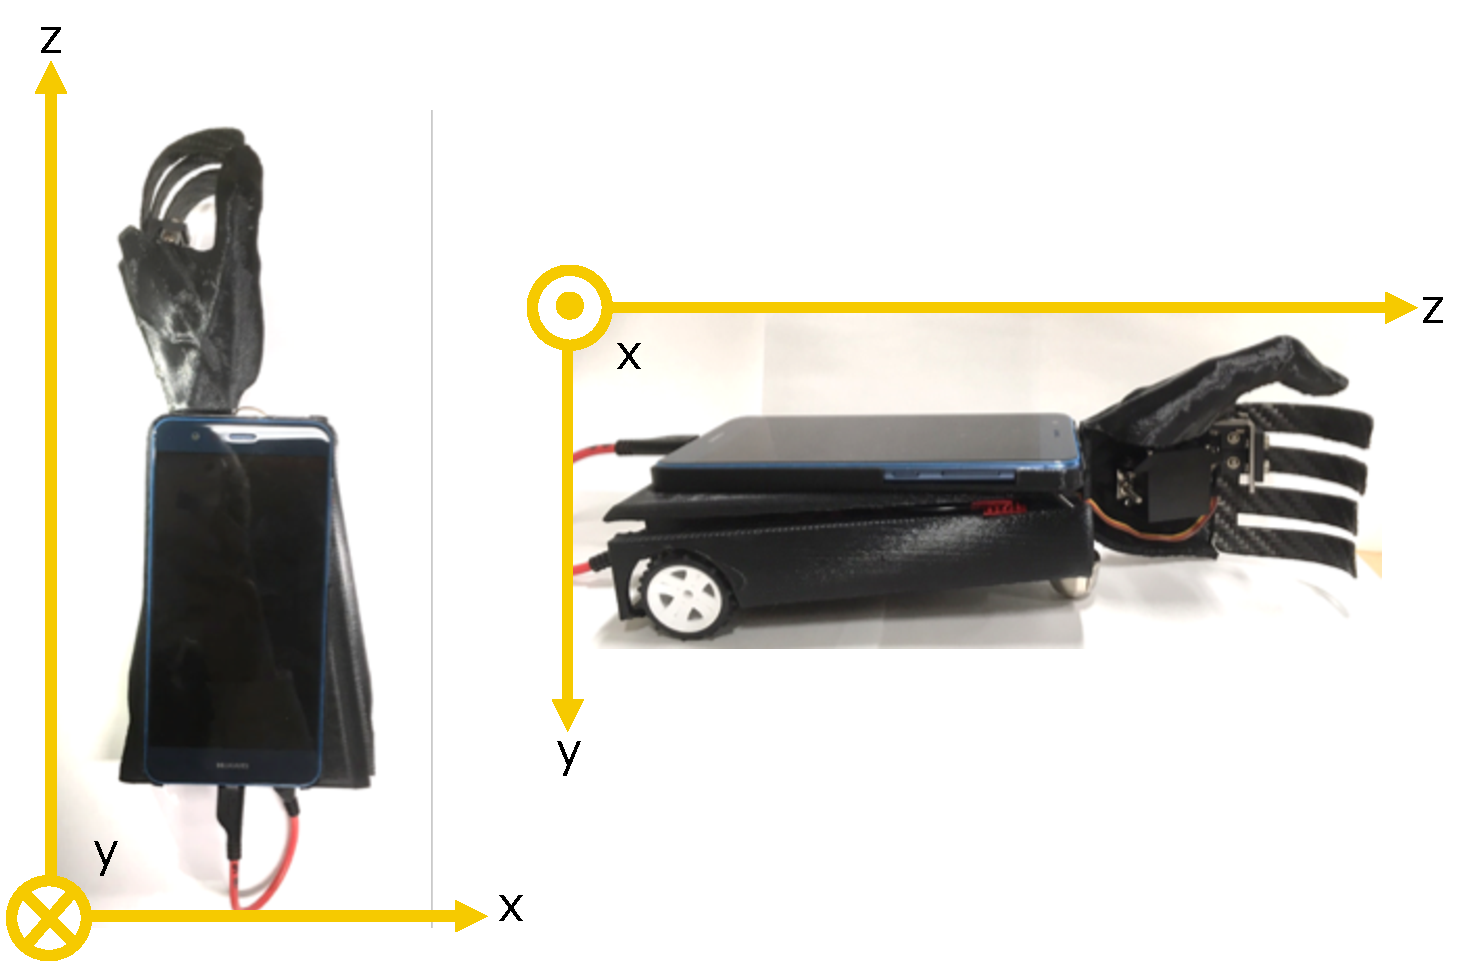
\includegraphics[width=0.9\linewidth]{figure/chapter3/1号機向き}
        \caption{Definition of orientation at protoptype No.1}
        \label{fig:1号機向き}
    \end{minipage}
\end{figure}


\subsection{学習と結果}
1号機の行うタスクとして接近タスクを行った.実機で2日間に渡り約300episodes学習させた.その学習の中で成功したepisodeにおけるロボットの挙動を\fig{1号機例}に示す.まず,旋回することであたりを探索する.カメラにターゲットを捉えたらそれに向かって接近し,一定の距離まで近づいたら把持を行う.このような流れで学習が進んでいることが示唆された.

\begin{figure}[H]
    \centering
    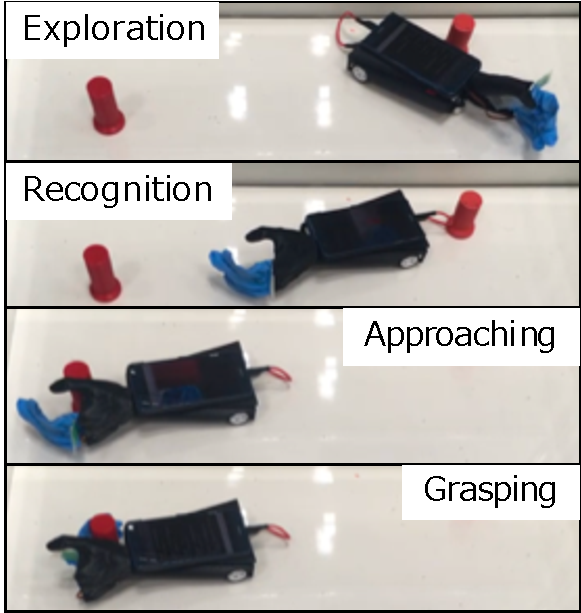
\includegraphics[width=0.7\linewidth]{figure/chapter3/robothand-v1_demo}
    \caption{Demonstration of prototype No.1 at sucess episode.}
    \label{fig:1号機例}
\end{figure}

しかしカメラのフレームレート(frame per second: fps)が低く1fps程度であり,各stepにおける行動が1秒程度持続してしまい,同じ場所を旋回しつづける行動が問題であった.fpsが低い原因として,スマートフォンのカメラにプロテクトがかかっておりビデオが使えず,カメラの単写を使用せざるを得ないことが挙げられる.またスマートフォンの演算能力ではより高次元の状態や行動を入出力とした強化学習は難しいため,"曲がりながら進む"といった前進と旋回の組み合わせができなかった.


\section{物理シミュレーション}
強化学習では学習に多くの時間がかかる.また実機ではバッテリー残量や壁にぶつかった際に位置を人の手で直す必要がある.そこでより学習を進めかつ自動で学習ループを回すために物理シミュレーションを用いた.これにより学習過程を常に記録・参照することもできる.


\subsection{評価手法}
シミュレーション物理エンジンとしてBullet Physics Engineを用いた.実装においてはAPIがPythonで用意されているPyBullet\cite{pybullet}を使用した.\fig{1号機simu}にCADで作製したロボットハンドをシミュレーション環境にレンダリングした画像を示す.

\begin{figure}[H]
    \centering
    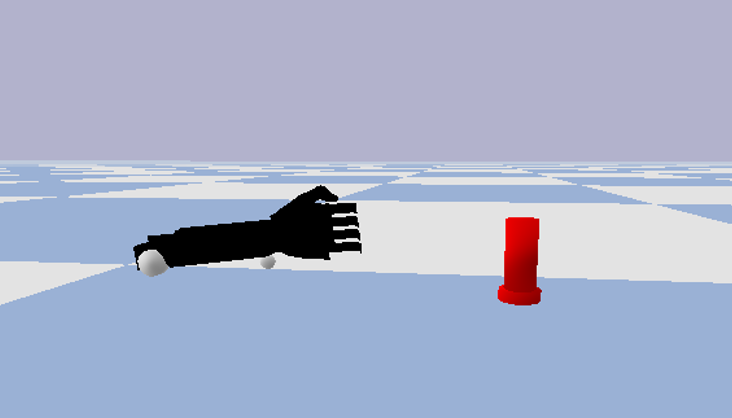
\includegraphics[width=0.7\linewidth]{figure/chapter3/bullet_demo}
    \caption{Environment of bullet physics simulation.}
    \label{fig:1号機simu}
\end{figure}

ターゲットをランダムに配置し,観測状態と報酬を変えて学習がどのように進むかを実験した.タスクとしては接近のみを行い,ルールベース化してある把持は省略した.性能をテストする際,$\epsilon$-greedy方策の探索する確率を0とし,greedy方策でテストする.そして10episodeごとに報酬の総和を計算し,1episodeあたりの報酬として平均をとった.


\subsection{結果}
まず,状態としてカメラから認識できるターゲットの面積値(最大を100に規格化),及びそのフレーム間差分の2次元を与えた.また報酬として,タスクが成功したら+1,1episode以内に成功しなかったら-1,各stepでは0とし,学習を行った(\fig{報酬離散}).Episodeが経過しても報酬に変化がないことから,学習が収束していないことがわかる.この原因としては観測が良くないかまたは報酬設計が悪いかの2つが考えられる.Agentの行動は環境から得られる報酬に依ることを考慮すると,多くのepisode学習を行っても収束しないということは観測状態が良くないと考えられる.また,報酬は連続値で与える方が各episodeごとではなく各stepごとにパラメータ更新が行えるため学習がスムーズに進むので,報酬を連続値に変えた.

次に,状態としてロボットハンドとターゲットとの相対位置$(x,y)$座標の2次元を与えた.また報酬として,ターゲットとの距離を与え,学習を行った(\fig{報酬距離}).\fig{報酬離散}とは挙動が異なり,初めの数10episodeで急激に報酬が増加し,その後横ばいとなっていることがわかる.Episodeを重ねても報酬は飽和しているため,学習が収束していることがわかる.このパラメータでレンダリングして確認してみると,学習が成功していることが分かった.

また,状態としては先ほどと同様に相対位置$(x,y)$座標の2次元を与え,報酬としてターゲットの面積値を与え学習を行った(\fig{報酬面積}).Episodeが進むとなだらかに報酬が増加し,400episode付近から報酬が飽和していることがわかる.このことから学習が収束していると言える.このパラメータでレンダリングして確認してみると,確かに学習が成功していることが分かった.

\begin{figure}
    \centering
    \begin{minipage}[t]{0.45\linewidth}
        \centering
        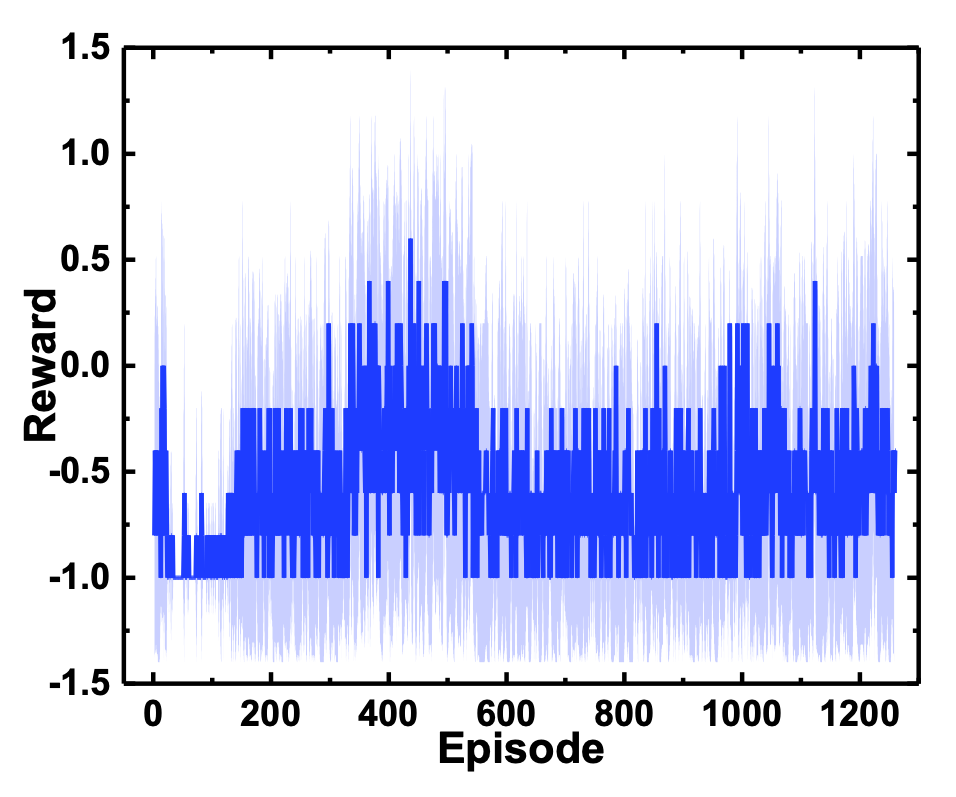
\includegraphics[width=\linewidth]{figure/chapter3/rew=01_obs=面積重心_origin}
        \subcaption{State: area of target, time difference of the area; Reward: success=1, failure=-1, others=0.}
        \label{fig:報酬離散}
    \end{minipage}
    \hspace*{\fill}
    \begin{minipage}[t]{0.45\linewidth}
        \centering
        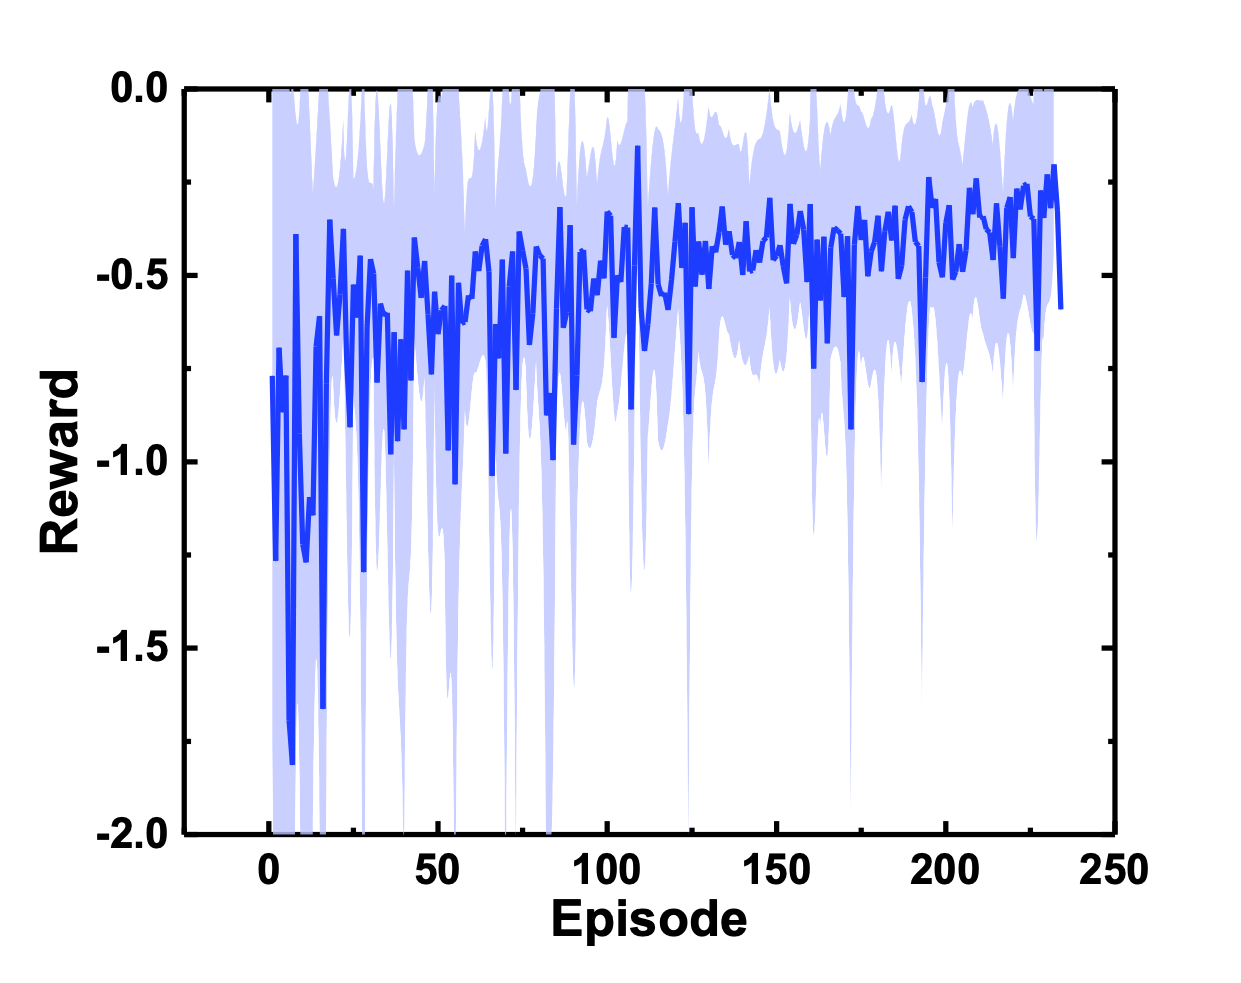
\includegraphics[width=1.1\linewidth]{figure/chapter3/QL_rew=distance_obs=posvec_origin}
        \subcaption{State: relative position; Reward: distance between agent and target.}
        \label{fig:報酬距離}
    \end{minipage}
    \begin{minipage}[t]{0.5\linewidth}
        \centering
        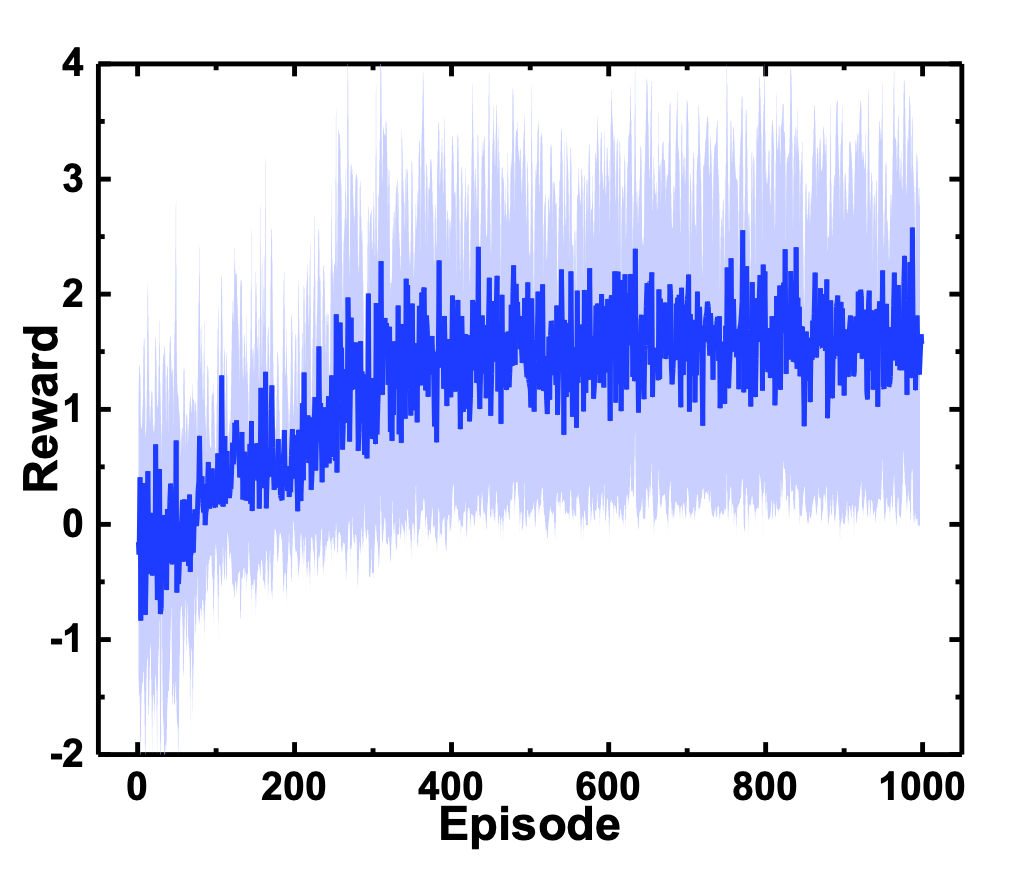
\includegraphics[width=0.95\linewidth]{figure/chapter3/QL_rew=redArea_obs=posvec_origin}
        \subcaption{State: relative position; Reward: area of target.}
        \label{fig:報酬面積}
    \end{minipage}
    \caption{Learning curve of each state and reward at simulation.}
    \label{fig:シミュレーション結果}
\end{figure}


\subsection{考察}
結果を踏まえると,報酬はタスクの成否にあまり関係なく,環境を正しく観測することが重要だということが分かった.\fig{報酬離散}の状態は言い換えると一人称視点であり,\fig{報酬距離},\fig{報酬面積}は環境を俯瞰して見る三人称視点である.三人称視点では自分の周囲の環境全体を観測することができるが,一人称視点では自分が向いている方向しか観測できない.すなわち,探索をしていく中でターゲットを捉えることが必然的に少なくなり,報酬による行動の評価が難しくなる.したがって,一人称視点では中々学習が進まず,三人称視点ではスムーズに報酬が飽和し,学習が完了したと考えられる.


\section{まとめ}
自己完結型の自律駆動ロボットハンドを実現するため,全てのシステムを人間の手のサイズに収容することを目指してスマートフォンのCPU,アクチュエータ制御インターフェースとスマートフォンのカメラ(環境認識)を用いたロボットハンドを作製した.
指定した色(赤色)の物体を認識し,接近し,把持するという一連の動作を行システムを開発し,ターゲットに接近し把持することに成功した.実機での学習とシミュレーション環境での学習を両方行い,外部環境をどう状態に落とし込み状態とするかが学習に大きく関わることを示した.そして,接近タスクにおいてはロボットハンド視点では学習が収束せず,ロボットハンド視点と共にターゲットを俯瞰する視点を併用して観測すると正しく学習できることがわかった.

1号機の課題として以下が挙げられる.
機械的な自由度が少なく,様々な形状の物体を持ち上げて運ぶことが難しい.
様々な種類の物体を識別できない.
AndroidのスマートフォンではPythonから制御すると内蔵カメラの動画が使えず,リアルタイム性に欠ける.
スマートフォンの計算リソースでは重い画像処理が不可能である.

今後は,物体を把持した後に次の行為を実行させるため,より自由度を上げ複雑な動作を可能にするロボットハンドを開発する事の必要性を実感した.ロボットの制御精度と動作速度向上には,環境を認識するセンサとして,環境を俯瞰する位置に定点カメラを設置したり,作動環境内に測距センサを配置する必要がある.加えて,把持対象物が複数ある場合に,使用者が意図する物体を正しく認識し把持できる物体識別性能が重要になってくる.

茨城県立大学付属病院リハビリテーション科にて義手使用患者へヒアリングを行い,ロボットハンド1号機の感想をいただいた.
\begin{itemize}
    \item "軽いと感じた"
    \item "家に帰ったらテーブルの上で作業することが多いから,ロボットハンドの有用性はあると思う"
    \item "自分のスマートフォンでできるのが良い"
    \item "クラウドを使わないから停電になったときでも使えて良い"
\end{itemize}
このように義手使用患者からも好評であり,本システムの実用性は高いと考える.

